

\tikzset{every picture/.style={line width=0.75pt}} %set default line width to 0.75pt        

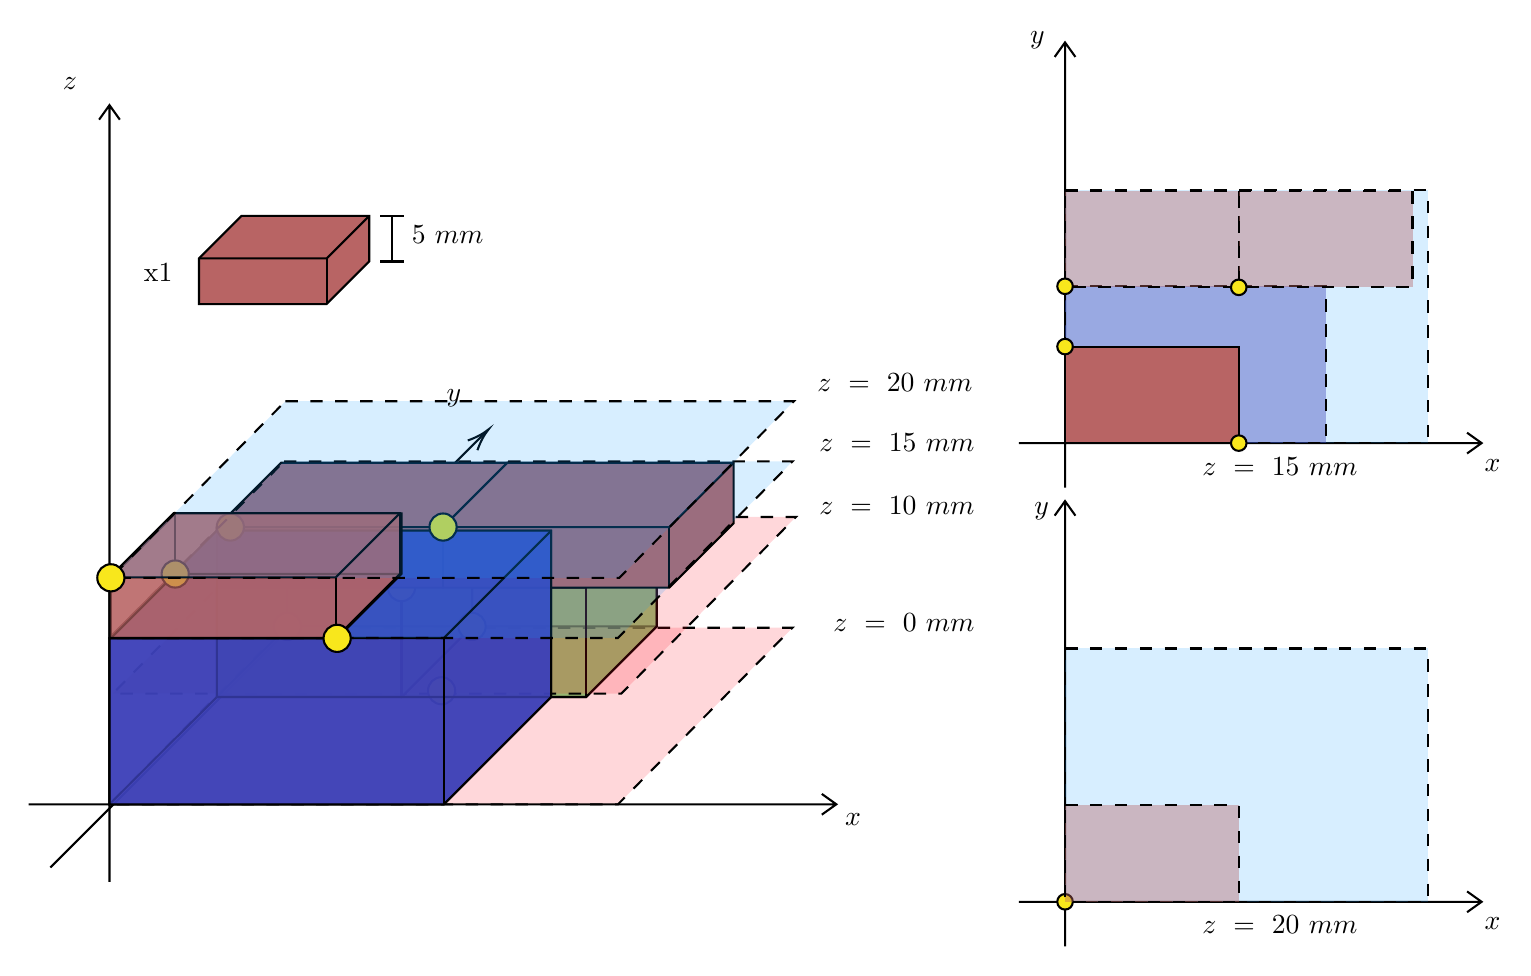
\begin{tikzpicture}[x=0.75pt,y=0.75pt,yscale=-1,xscale=1]
%uncomment if require: \path (0,511); %set diagram left start at 0, and has height of 511

%Shape: Cube [id:dp13382747579819188] 
\draw  [fill={rgb, 255:red, 130; green, 184; blue, 100 }  ,fill opacity=0.63 ] (400.59,311.37) -- (366.58,345.38) -- (277.6,345.38) -- (277.6,292.66) -- (311.6,258.65) -- (400.59,258.65) -- cycle ; \draw   (277.6,345.38) -- (311.6,311.37) -- (400.59,311.37) ; \draw   (311.6,311.37) -- (311.6,258.65) ;
%Shape: Parallelogram [id:dp6966422926494509] 
\draw  [fill={rgb, 255:red, 255; green, 17; blue, 34 }  ,fill opacity=0.17 ][dash pattern={on 4.5pt off 4.5pt}] (221,312) -- (466,312) -- (381.91,397.07) -- (136.91,397.07) -- cycle ;
%Shape: Cube [id:dp7954856505993868] 
\draw  [fill={rgb, 255:red, 130; green, 184; blue, 100 }  ,fill opacity=0.63 ] (277.6,292.66) -- (311.6,258.65) -- (400.59,258.65) -- (400.59,311.37) -- (366.58,345.38) -- (277.6,345.38) -- cycle ; \draw   (400.59,258.65) -- (366.58,292.66) -- (277.6,292.66) ; \draw   (366.58,292.66) -- (366.58,345.38) ;
%Shape: Parallelogram [id:dp4537315333431484] 
\draw  [fill={rgb, 255:red, 255; green, 17; blue, 34 }  ,fill opacity=0.17 ][dash pattern={on 4.5pt off 4.5pt}] (222.62,258.65) -- (467.62,258.65) -- (383.53,343.73) -- (138.53,343.73) -- cycle ;
%Shape: Axis 2D [id:dp9498145046786112] 
\draw  (98,397.07) -- (487.11,397.07)(136.91,60.22) -- (136.91,434.5) (480.11,392.07) -- (487.11,397.07) -- (480.11,402.07) (131.91,67.22) -- (136.91,60.22) -- (141.91,67.22)  ;
%Straight Lines [id:da4658635517686608] 
\draw    (108.47,427.52) -- (318.19,217.8) ;
\draw [shift={(319.6,216.39)}, rotate = 135] [color={rgb, 255:red, 0; green, 0; blue, 0 }  ][line width=0.75]    (10.93,-3.29) .. controls (6.95,-1.4) and (3.31,-0.3) .. (0,0) .. controls (3.31,0.3) and (6.95,1.4) .. (10.93,3.29)   ;
%Shape: Cube [id:dp037325029593255565] 
\draw  [fill={rgb, 255:red, 184; green, 100; blue, 100 }  ,fill opacity=1 ] (180.05,134.05) -- (200.55,113.55) -- (262.05,113.55) -- (262.05,135.55) -- (241.55,156.05) -- (180.05,156.05) -- cycle ; \draw   (262.05,113.55) -- (241.55,134.05) -- (180.05,134.05) ; \draw   (241.55,134.05) -- (241.55,156.05) ;
%Straight Lines [id:da907575610680141] 
\draw    (273.05,113.55) -- (273.05,135.55) ;
\draw [shift={(273.05,135.55)}, rotate = 270] [color={rgb, 255:red, 0; green, 0; blue, 0 }  ][line width=0.75]    (0,5.59) -- (0,-5.59)   ;
\draw [shift={(273.05,113.55)}, rotate = 270] [color={rgb, 255:red, 0; green, 0; blue, 0 }  ][line width=0.75]    (0,5.59) -- (0,-5.59)   ;
%Shape: Cube [id:dp07109550183608815] 
\draw  [fill={rgb, 255:red, 130; green, 184; blue, 100 }  ,fill opacity=0.63 ] (311.6,311.37) -- (277.6,345.38) -- (188.61,345.38) -- (188.61,292.66) -- (222.62,258.65) -- (311.6,258.65) -- cycle ; \draw   (188.61,345.38) -- (222.62,311.37) -- (311.6,311.37) ; \draw   (222.62,311.37) -- (222.62,258.65) ;
%Shape: Cube [id:dp004470545573486695] 
\draw  [fill={rgb, 255:red, 130; green, 184; blue, 100 }  ,fill opacity=0.63 ] (188.61,292.66) -- (222.62,258.65) -- (311.6,258.65) -- (311.6,311.37) -- (277.6,345.38) -- (188.61,345.38) -- cycle ; \draw   (311.6,258.65) -- (277.6,292.66) -- (188.61,292.66) ; \draw   (277.6,292.66) -- (277.6,345.38) ;
%Shape: Ellipse [id:dp6668747084579564] 
\draw  [fill={rgb, 255:red, 248; green, 231; blue, 28 }  ,fill opacity=1 ] (216.07,311.37) .. controls (216.07,307.75) and (219,304.82) .. (222.62,304.82) .. controls (226.23,304.82) and (229.16,307.75) .. (229.16,311.37) .. controls (229.16,314.98) and (226.23,317.91) .. (222.62,317.91) .. controls (219,317.91) and (216.07,314.98) .. (216.07,311.37) -- cycle ;
%Shape: Axis 2D [id:dp44476464107887725] 
\draw  (575,223.05) -- (798,223.05)(597.3,30) -- (597.3,244.5) (791,218.05) -- (798,223.05) -- (791,228.05) (592.3,37) -- (597.3,30) -- (602.3,37)  ;
%Shape: Rectangle [id:dp8842448402236128] 
\draw  [fill={rgb, 255:red, 17; green, 154; blue, 255 }  ,fill opacity=0.17 ][dash pattern={on 4.5pt off 4.5pt}] (597.3,101) -- (772,101) -- (772,223.05) -- (597.3,223.05) -- cycle ;
%Shape: Rectangle [id:dp22549871314391357] 
\draw  [fill={rgb, 255:red, 61; green, 65; blue, 184 }  ,fill opacity=0.4 ][dash pattern={on 4.5pt off 4.5pt}] (597.3,147.5) -- (723,147.5) -- (723,223.05) -- (597.3,223.05) -- cycle ;
%Shape: Ellipse [id:dp8550857930670437] 
\draw  [fill={rgb, 255:red, 248; green, 231; blue, 28 }  ,fill opacity=1 ] (305.06,311.37) .. controls (305.06,307.75) and (307.99,304.82) .. (311.6,304.82) .. controls (315.22,304.82) and (318.15,307.75) .. (318.15,311.37) .. controls (318.15,314.98) and (315.22,317.91) .. (311.6,317.91) .. controls (307.99,317.91) and (305.06,314.98) .. (305.06,311.37) -- cycle ;
%Shape: Ellipse [id:dp09363312581695205] 
\draw  [fill={rgb, 255:red, 248; green, 231; blue, 28 }  ,fill opacity=1 ] (271.05,292.66) .. controls (271.05,289.05) and (273.98,286.12) .. (277.6,286.12) .. controls (281.21,286.12) and (284.14,289.05) .. (284.14,292.66) .. controls (284.14,296.28) and (281.21,299.21) .. (277.6,299.21) .. controls (273.98,299.21) and (271.05,296.28) .. (271.05,292.66) -- cycle ;
%Shape: Ellipse [id:dp7691678960010918] 
\draw  [fill={rgb, 255:red, 248; green, 231; blue, 28 }  ,fill opacity=1 ] (290.37,342.37) .. controls (290.37,338.76) and (293.3,335.83) .. (296.91,335.83) .. controls (300.52,335.83) and (303.45,338.76) .. (303.45,342.37) .. controls (303.45,345.98) and (300.52,348.91) .. (296.91,348.91) .. controls (293.3,348.91) and (290.37,345.98) .. (290.37,342.37) -- cycle ;
%Shape: Cube [id:dp0837514121075894] 
\draw  [fill={rgb, 255:red, 184; green, 100; blue, 100 }  ,fill opacity=1 ] (188.61,263.5) -- (219.61,232.5) -- (328.63,232.5) -- (328.63,261.66) -- (297.63,292.66) -- (188.61,292.66) -- cycle ; \draw   (328.63,232.5) -- (297.63,263.5) -- (188.61,263.5) ; \draw   (297.63,263.5) -- (297.63,292.66) ;
%Shape: Cube [id:dp22596641921194294] 
\draw  [fill={rgb, 255:red, 184; green, 100; blue, 100 }  ,fill opacity=1 ] (297.63,263.5) -- (328.63,232.5) -- (437.65,232.5) -- (437.65,261.66) -- (406.65,292.66) -- (297.63,292.66) -- cycle ; \draw   (437.65,232.5) -- (406.65,263.5) -- (297.63,263.5) ; \draw   (406.65,263.5) -- (406.65,292.66) ;
%Shape: Cube [id:dp9390528785176023] 
\draw  [fill={rgb, 255:red, 61; green, 65; blue, 184 }  ,fill opacity=0.8 ] (349.7,345.38) -- (298,397.07) -- (136.91,397.07) -- (136.91,316.94) -- (188.61,265.25) -- (349.7,265.25) -- cycle ; \draw   (136.91,397.07) -- (188.61,345.38) -- (349.7,345.38) ; \draw   (188.61,345.38) -- (188.61,265.25) ;
%Shape: Cube [id:dp4332809548010883] 
\draw  [fill={rgb, 255:red, 61; green, 65; blue, 184 }  ,fill opacity=0.8 ] (136.91,316.94) -- (188.61,265.25) -- (349.7,265.25) -- (349.7,345.38) -- (298,397.07) -- (136.91,397.07) -- cycle ; \draw   (349.7,265.25) -- (298,316.94) -- (136.91,316.94) ; \draw   (298,316.94) -- (298,397.07) ;
%Shape: Ellipse [id:dp8530820745955504] 
\draw  [fill={rgb, 255:red, 248; green, 231; blue, 28 }  ,fill opacity=1 ] (188.61,263.5) .. controls (188.61,259.89) and (191.54,256.96) .. (195.15,256.96) .. controls (198.77,256.96) and (201.69,259.89) .. (201.69,263.5) .. controls (201.69,267.11) and (198.77,270.04) .. (195.15,270.04) .. controls (191.54,270.04) and (188.61,267.11) .. (188.61,263.5) -- cycle ;
%Shape: Ellipse [id:dp7570025851179228] 
\draw  [fill={rgb, 255:red, 248; green, 231; blue, 28 }  ,fill opacity=1 ] (291.09,263.5) .. controls (291.09,259.89) and (294.02,256.96) .. (297.63,256.96) .. controls (301.24,256.96) and (304.17,259.89) .. (304.17,263.5) .. controls (304.17,267.11) and (301.24,270.04) .. (297.63,270.04) .. controls (294.02,270.04) and (291.09,267.11) .. (291.09,263.5) -- cycle ;
%Shape: Parallelogram [id:dp8088836688018484] 
\draw  [fill={rgb, 255:red, 17; green, 154; blue, 255 }  ,fill opacity=0.17 ][dash pattern={on 4.5pt off 4.5pt}] (221,231.87) -- (466,231.87) -- (381.91,316.94) -- (136.91,316.94) -- cycle ;
%Shape: Rectangle [id:dp8807699745453305] 
\draw  [fill={rgb, 255:red, 184; green, 100; blue, 100 }  ,fill opacity=0.4 ][dash pattern={on 4.5pt off 4.5pt}] (597.3,101.5) -- (681,101.5) -- (681,148) -- (597.3,148) -- cycle ;
%Shape: Rectangle [id:dp7105108279475557] 
\draw  [fill={rgb, 255:red, 184; green, 100; blue, 100 }  ,fill opacity=0.4 ][dash pattern={on 4.5pt off 4.5pt}] (681,101.5) -- (764.7,101.5) -- (764.7,148) -- (681,148) -- cycle ;
%Shape: Circle [id:dp7943424960137139] 
\draw  [fill={rgb, 255:red, 248; green, 231; blue, 28 }  ,fill opacity=1 ] (593.55,147.5) .. controls (593.55,145.43) and (595.23,143.75) .. (597.3,143.75) .. controls (599.37,143.75) and (601.05,145.43) .. (601.05,147.5) .. controls (601.05,149.57) and (599.37,151.25) .. (597.3,151.25) .. controls (595.23,151.25) and (593.55,149.57) .. (593.55,147.5) -- cycle ;
%Shape: Circle [id:dp9005405536776231] 
\draw  [fill={rgb, 255:red, 248; green, 231; blue, 28 }  ,fill opacity=1 ] (677.25,148) .. controls (677.25,145.93) and (678.93,144.25) .. (681,144.25) .. controls (683.07,144.25) and (684.75,145.93) .. (684.75,148) .. controls (684.75,150.07) and (683.07,151.75) .. (681,151.75) .. controls (678.93,151.75) and (677.25,150.07) .. (677.25,148) -- cycle ;
%Shape: Cube [id:dp653646926223087] 
\draw  [fill={rgb, 255:red, 184; green, 100; blue, 100 }  ,fill opacity=0.67 ] (277.6,286.12) -- (246.6,317.12) -- (137.57,317.12) -- (137.57,287.96) -- (168.57,256.96) -- (277.6,256.96) -- cycle ; \draw   (137.57,317.12) -- (168.57,286.12) -- (277.6,286.12) ; \draw   (168.57,286.12) -- (168.57,256.96) ;
%Shape: Ellipse [id:dp6705610706320286] 
\draw  [fill={rgb, 255:red, 248; green, 231; blue, 28 }  ,fill opacity=1 ] (162.03,286.12) .. controls (162.03,282.51) and (164.96,279.58) .. (168.57,279.58) .. controls (172.19,279.58) and (175.12,282.51) .. (175.12,286.12) .. controls (175.12,289.73) and (172.19,292.66) .. (168.57,292.66) .. controls (164.96,292.66) and (162.03,289.73) .. (162.03,286.12) -- cycle ;
%Shape: Cube [id:dp7235035205502207] 
\draw  [fill={rgb, 255:red, 184; green, 100; blue, 100 }  ,fill opacity=0.67 ] (136.91,287.78) -- (167.91,256.78) -- (276.93,256.78) -- (276.93,285.94) -- (245.93,316.94) -- (136.91,316.94) -- cycle ; \draw   (276.93,256.78) -- (245.93,287.78) -- (136.91,287.78) ; \draw   (245.93,287.78) -- (245.93,316.94) ;
%Shape: Ellipse [id:dp5459811026373071] 
\draw  [fill={rgb, 255:red, 248; green, 231; blue, 28 }  ,fill opacity=1 ] (240.05,317.12) .. controls (240.05,313.51) and (242.98,310.58) .. (246.6,310.58) .. controls (250.21,310.58) and (253.14,313.51) .. (253.14,317.12) .. controls (253.14,320.73) and (250.21,323.66) .. (246.6,323.66) .. controls (242.98,323.66) and (240.05,320.73) .. (240.05,317.12) -- cycle ;
%Shape: Parallelogram [id:dp6357278096082768] 
\draw  [fill={rgb, 255:red, 17; green, 154; blue, 255 }  ,fill opacity=0.17 ][dash pattern={on 4.5pt off 4.5pt}] (221.66,202.88) -- (466.66,202.88) -- (382.57,287.96) -- (137.57,287.96) -- cycle ;
%Shape: Ellipse [id:dp5454534055037792] 
\draw  [fill={rgb, 255:red, 248; green, 231; blue, 28 }  ,fill opacity=1 ] (131.03,287.96) .. controls (131.03,284.34) and (133.96,281.41) .. (137.57,281.41) .. controls (141.19,281.41) and (144.12,284.34) .. (144.12,287.96) .. controls (144.12,291.57) and (141.19,294.5) .. (137.57,294.5) .. controls (133.96,294.5) and (131.03,291.57) .. (131.03,287.96) -- cycle ;
%Shape: Axis 2D [id:dp13890777694672107] 
\draw  (575,444.05) -- (798,444.05)(597.3,251) -- (597.3,465.5) (791,439.05) -- (798,444.05) -- (791,449.05) (592.3,258) -- (597.3,251) -- (602.3,258)  ;
%Shape: Rectangle [id:dp5079067412188037] 
\draw  [fill={rgb, 255:red, 17; green, 154; blue, 255 }  ,fill opacity=0.17 ][dash pattern={on 4.5pt off 4.5pt}] (597.3,322) -- (772,322) -- (772,444.05) -- (597.3,444.05) -- cycle ;
%Shape: Circle [id:dp4515950519247576] 
\draw  [fill={rgb, 255:red, 248; green, 231; blue, 28 }  ,fill opacity=1 ] (593.55,444.05) .. controls (593.55,441.98) and (595.23,440.3) .. (597.3,440.3) .. controls (599.37,440.3) and (601.05,441.98) .. (601.05,444.05) .. controls (601.05,446.12) and (599.37,447.8) .. (597.3,447.8) .. controls (595.23,447.8) and (593.55,446.12) .. (593.55,444.05) -- cycle ;
%Shape: Rectangle [id:dp8775041721420133] 
\draw  [fill={rgb, 255:red, 184; green, 100; blue, 100 }  ,fill opacity=0.4 ][dash pattern={on 4.5pt off 4.5pt}] (597.3,397.55) -- (681,397.55) -- (681,444.05) -- (597.3,444.05) -- cycle ;
%Shape: Rectangle [id:dp19056688106305508] 
\draw  [fill={rgb, 255:red, 184; green, 100; blue, 100 }  ,fill opacity=1 ] (597.3,176.55) -- (681,176.55) -- (681,223.05) -- (597.3,223.05) -- cycle ;
%Shape: Circle [id:dp3722307923482907] 
\draw  [fill={rgb, 255:red, 248; green, 231; blue, 28 }  ,fill opacity=1 ] (593.55,176.55) .. controls (593.55,174.48) and (595.23,172.8) .. (597.3,172.8) .. controls (599.37,172.8) and (601.05,174.48) .. (601.05,176.55) .. controls (601.05,178.62) and (599.37,180.3) .. (597.3,180.3) .. controls (595.23,180.3) and (593.55,178.62) .. (593.55,176.55) -- cycle ;
%Shape: Circle [id:dp8906369239154822] 
\draw  [fill={rgb, 255:red, 248; green, 231; blue, 28 }  ,fill opacity=1 ] (677.25,223.05) .. controls (677.25,220.98) and (678.93,219.3) .. (681,219.3) .. controls (683.07,219.3) and (684.75,220.98) .. (684.75,223.05) .. controls (684.75,225.12) and (683.07,226.8) .. (681,226.8) .. controls (678.93,226.8) and (677.25,225.12) .. (677.25,223.05) -- cycle ;

% Text Node
\draw (484.19,303.66) node [anchor=north west][inner sep=0.75pt]    {$z\ =\ 0\ mm$};
% Text Node
\draw (297.9,195.7) node [anchor=north west][inner sep=0.75pt]    {$y$};
% Text Node
\draw (489.84,399.85) node [anchor=north west][inner sep=0.75pt]    {$x$};
% Text Node
\draw (112.94,45.64) node [anchor=north west][inner sep=0.75pt]    {$z$};
% Text Node
\draw (152,135) node [anchor=north west][inner sep=0.75pt]   [align=left] {x1};
% Text Node
\draw (281.05,116.95) node [anchor=north west][inner sep=0.75pt]    {$5\ mm$};
% Text Node
\draw (477.48,217.2) node [anchor=north west][inner sep=0.75pt]    {$z\ =\ 15\ mm$};
% Text Node
\draw (798,229.4) node [anchor=north west][inner sep=0.75pt]    {$x$};
% Text Node
\draw (662,228.4) node [anchor=north west][inner sep=0.75pt]    {$z\ =\ 15\ mm$};
% Text Node
\draw (477.48,247.2) node [anchor=north west][inner sep=0.75pt]    {$z\ =\ 10\ mm$};
% Text Node
\draw (476.48,188.2) node [anchor=north west][inner sep=0.75pt]    {$z\ =\ 20\ mm$};
% Text Node
\draw (798,450.4) node [anchor=north west][inner sep=0.75pt]    {$x$};
% Text Node
\draw (662,449.4) node [anchor=north west][inner sep=0.75pt]    {$z\ =\ 20\ mm$};
% Text Node
\draw (581,250.4) node [anchor=north west][inner sep=0.75pt]    {$y$};
% Text Node
\draw (579,23.4) node [anchor=north west][inner sep=0.75pt]    {$y$};


\end{tikzpicture}
